\renewcommand{\lastmod}{September 26, 2023}
\renewcommand{\chapterauthors}{Markus Lippitz}

\chapter{Gaussian Beams}


\goal{By the end of this chapter you should be able to explain the electric field in a Gaussian focus.
You can construct a Gaussian beam 'by hand' for typical lens systems and calculate it using the ABCD law.}


\section{Overview}

We extend our model to describe light. In this and the following chapters we will use wave optics and assume that light is a scalar wave. We will introduce typical wave functions as plane and spherical waves. Of particular importance are Gaussian beams: as eigenmodes of a laser resonator, they are ubiquitous in optical experiments. We will discuss how these waves and beams are transmitted through optical elements and how we can determine their properties.
More details on these topics can be found in chapter 2 and 3 of \cite{SalehTeich1991}, chapter 4.6 of \cite{Hering_Martin_Optik},  chapter 13 of \cite{Hecht_Optics}.



%-----------------------------------------------------------------------------
\section{Postulates of Wave Optics}

The wave function $u(\br, t)$ is complex-valued and fulfills the wave equation
\begin{equation}
    \nabla^2 u - \frac{1}{c^2} \, \frac{\partial^2 u}{\partial t^2} = 0
\end{equation}
with $c = c_0 /n$ the velocity of light in the medium of refractive index $n$. 
We do not yet assign a physical meaning to the wave function $u(\br, t)$. But since you have seen Maxwell's equations elsewhere, you might think of it as one component of the electric field, for example. At interfaces between media, the index of refraction $n$ changes and thus also $1/c$, but we still do not discuss the physics of such interfaces and partial reflection is beyond our scope.
The only connection we make to observable physical quantities is by defining the  \emph{intensity} $I$ of the wave as
\begin{equation}
    I(\br) = \braket{ |u(\br, t) |^2 }
\end{equation}
where the pointed brackets indicate a time average over a period long compared to the wave period.

A consequence of the linear wave equation is the superposition principle. If $u$ and $v$ are solutions to the wave equation, then also $\alpha u + \beta v$ is a solution. This also means that light beams cross themselves without interaction.


\section{Monochromatic waves}

The solutions of the wave equation can be written as harmonic functions
\begin{equation}
    u(\br, t)  = \tilde{u}(\br) \, e^{- i \omega t}
\end{equation}
with an angular frequency $\omega = 2 \pi \nu$. The spatial part $\tilde{u}(\br)$ fulfils the Helmholtz equation
\begin{equation}
    \nabla^2 \tilde{u} + k^2 \tilde{u} = 0 \quad \text{with} \quad k = \frac{\omega}{c}
\end{equation}
$k$ is called the \emph{wavenumber} and becomes the \emph{wavevector} when going to three dimensions. The intensity is then given by $\tilde{u}(\br)$
\begin{equation}
    I(\br) = \braket{ |u(\br, t) |^2 } = |\tilde{u}(\br) |^2 \quad , 
\end{equation}
i.e., the intensity of a monochromatic wave is constant in time. 

Lets discuss a few typical examples

\paragraph*{Plane wave} The amplitude $\tilde{u}$ is given by
\begin{equation}
 \tilde{u}(\br) = A \, e^{i \bk \cdot \br}
\end{equation}
with $\bk$ the wavevector and $|\bk| = k $. The \emph{wavefronts}, i.e., surfaces of constant phase $\phi = q \, 2 \pi =  \arg \tilde{u}(\br)$, are parallel and equidistant planes. The distance is the wavelength $\lambda = c / \nu = 2 \pi / k$.

When the index of refraction $n$ changes at an interface, the frequency $\omega$ remains the same, but the wavelength $\lambda$, the velocity of light $c$ and the wavenumber $k$ change
\begin{equation}
\lambda = \frac{\lambda_0}{n} \qquad
c = \frac{c_0}{n} \qquad
k = \frac{k_0}{n}
\end{equation}
 

\paragraph*{Spherical wave} Here the amplitude $\tilde{u}$ is given by
\begin{equation}
 \tilde{u}(\br) = \frac{A}{r} \, e^{i k r} \quad \text{with} \quad r = |\br|
 \label{eq:2_spherical_wave}
\end{equation}
Note that the right side of the equation does only use scalar variables. The wavefunction depends thus only on the distance to the origin and has spherical symmetry. The wavefronts are concentric spheres of distance $\lambda$.

\paragraph*{Paraboloidal wave} Close to the optical axis, we can approximate the spherical wave by a paraboloidal wave. We call $\theta$
\begin{equation}
    \theta^2 =  \frac{x^2 + y^2}{z^2} \ll 1
\end{equation}
and write $r$ as a Taylor expansion on $\theta$
\begin{align}
    r = & \sqrt{x^2 + y^2 + z^2}= z \sqrt{1 + \theta^2}
    = z \left( 1 + \frac{\theta^2}{2} - \frac{\theta^4}{8} + \cdots \right) \\
    \approx & z \left( 1 + \frac{\theta^2}{2} \right) = z + \frac{x^2 + y^2}{2z} 
\end{align}
This iis called the \emph{Fresnel approximation}. We put it into eq.  \ref{eq:2_spherical_wave} and approximate in the amplitude term even $r \approx z$. We get
\begin{equation}
    \tilde{u}(\br) = \frac{A}{z} \, e^{i k z} \, e^{i k \, \frac{x^2 + y^2}{2z}  }
\end{equation}
For points close to the optical axis but far from the origin, a spherical wave approaches a planar wave. In between, the paraboloidal wave is a useful approximation.


\begin{marginfigure}
    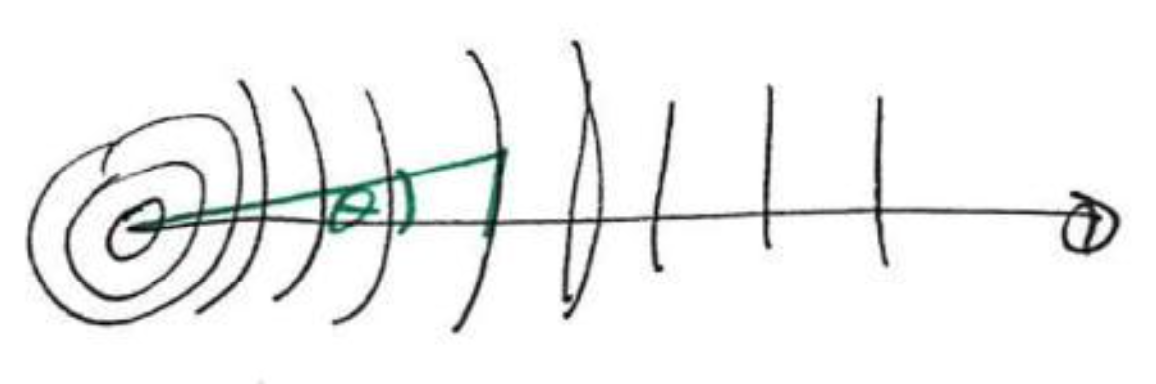
\includegraphics[width=\textwidth]{\currfiledir sketches/paraboloidal.png}
   \caption{XXX sketch Fig 2.2.4 S/T}
\end{marginfigure}


\section{A transparent plate}

As most simple optical element, we consider a transparent plate of thickness $d$ and index of refraction $n$ in air. We transmit a plane wave. The wavefunction is continuos at the interface. We are interested in the complex-valued transmission function $t(x,y)$
\begin{equation}
    t(x,y) = \frac{\tilde{u}(x,y,d)}{\tilde{u}(x,y,0)}
\end{equation}
For perpendicular incidence, the phase advances by $n k_0 d$ from left to right. The transmission function is thus
\begin{equation}
    t(x,y)  = e^{i n k_0 d}
\end{equation}

\begin{marginfigure}
    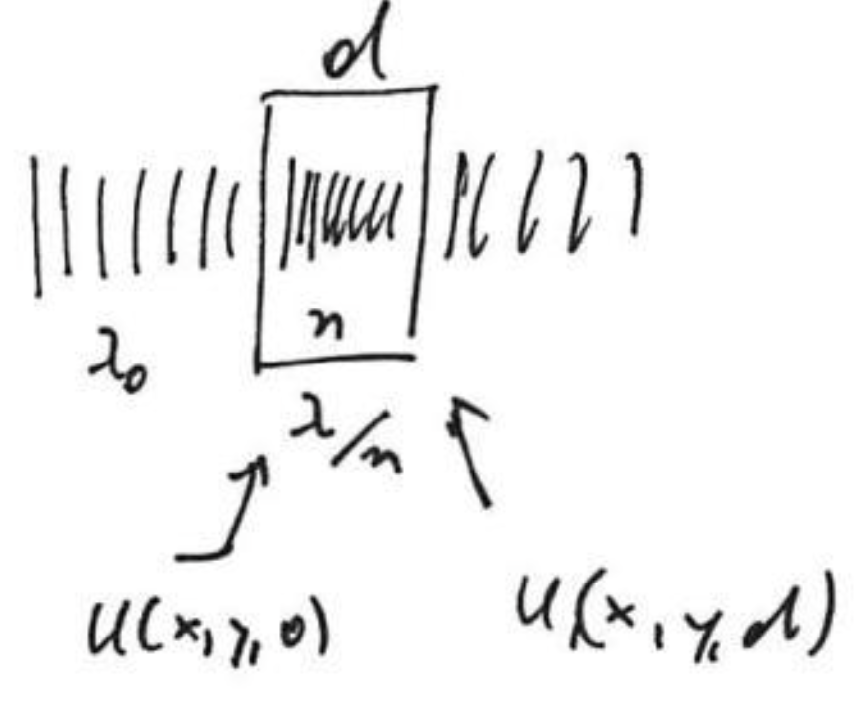
\includegraphics[width=\textwidth]{\currfiledir sketches/plate.png}
   \caption{A plate}
\end{marginfigure}


When the plane wave approaches the plate under angle $\theta$, then Snell's law gives the internal angle $\theta_i$ as $\sin \theta = n \sin \theta_i$. The wavevector makes this angle $\theta_i$ with the optical axis, so that the $z$-component of the term $\bk \cdot \br$ at the right side gives $n k \cos \theta_i$ and the total transmission function is
\begin{equation}
    t(x,y)  = e^{i n k_0 d \cos \theta_i}
\end{equation}
This is always against my intuition. The geometrical path in the plate gets longer by tilting it, but the phase difference becomes smaller. The point is that we only take the component along $z$ into account, as shifting a plane wave perpendicular to its direction of travel does not change anything.

We of course make again the approximation that the angle $\theta$ is small enough so that we can ignore the $\cos \theta_i$ part.

\begin{marginfigure}
    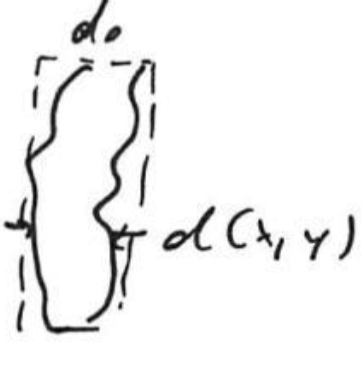
\includegraphics[width=0.5\textwidth]{\currfiledir sketches/plate_var_d.png}
   \caption{A plate of variable thickness}
\end{marginfigure}


If the plate has a variable thickness $d(x,y)$, we enclose it in a box of thickness $d_0$. Then part of the phase progression goes with $n$, part with air ($n=1$). In total this is
\begin{equation}
    t(x,y) \approx e^{i n k_0 d(x,y)} \,  e^{i k_0 (d_0 - d(x,y))}
    = h_0   e^{i (n-1) k_0 d(x,y)}
\end{equation}
with $h_0 = e^{i  k_0 d_0}$ a constant phase factor. This makes the approximation that all angles are small enough and neighboring parts of the plate do not 'mix' at the output.


\section{Conversion of a plane wave to a spherical wave by a lens}

\begin{marginfigure}
    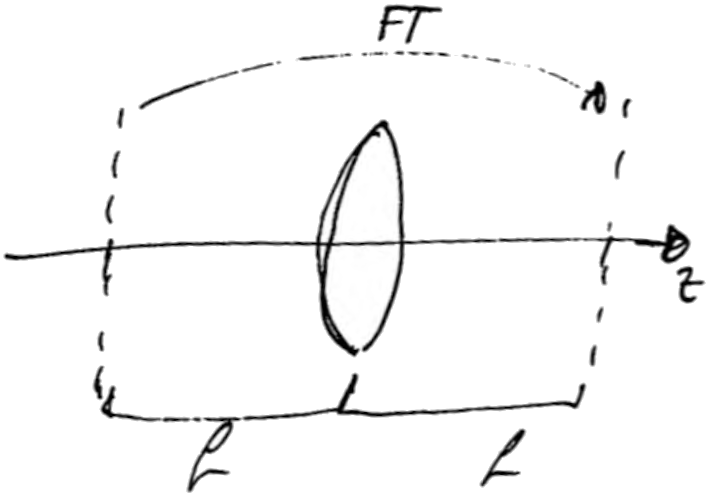
\includegraphics[width=\textwidth]{\currfiledir sketches/lens.png}
   \caption{A lens as plate of variable thickness}
\end{marginfigure}

The most interesting thin plate of variable thickness is a lens. For simplicity, we use a plane convex lens, i.e, set one radius of curvature to infinity. The thickness $d(x,y)$ of this plate is then
\begin{equation}
    d(x,y) = d_0 - \left( R - \sqrt{R^2 - (x^2 + y^2)} \right)
\end{equation}
We again use the Fresnel approximation $x^2 + y^2 \ll R^2$ and approximate the square-root term
\begin{equation}
    \sqrt{R^2 - (x^2 + y^2)}  = R \sqrt{1- \frac{x^2 + y^2}{R^2}} 
    \approx R \left( 1 -  \frac{x^2 + y^2}{2 R^2} \right)
\end{equation}
so that 
\begin{equation}
    d(x,y) \approx d_0 -  \frac{x^2 + y^2}{2 R^2}
\end{equation}
The transmission function is then
\begin{equation}
    t(x,y)= h_0 \,  e^{-i k_0 \frac{x^2 + y^2}{2f}}
    \quad 
    \text{with} \quad
    f = \frac{R}{n-1}
\end{equation}
and $h_0 = e^{i n k_0 d_0}$ another constant phase factor that we ignore.

A spherical lens thus transforms a plane wave into a paraboloidal wave centered around $z=f$.


\section{Gaussian beams as a paraxial solution of the wave equation}

When we have discussed typical solutions to the wave equation above, we started from the full wave equation, found spherical waves as solution, and then made the paraxial approximation to arrive at the paraboloidal waves. We could also have gone a different route. We can apply the paraxial approximation to the wave equation directly. This leads to the paraxial Helmholtz equation
\begin{equation}
    \nabla_T^2 A + i 2k \frac{\partial A}{\partial z} = 0
    \quad 
    \text{and}
    \quad
    \tilde{u}(\br) = A(\br) \, e^{i k z}
\end{equation}
with $ \nabla_T$ acting only on the transverse coordinates only. The envelop $ A(\br)$ modulates the carrier $\exp(i k z)$. $A$ needs to be \emph{slowly varying}, i.e., on a wavelength length scale it should not change much.

The paraboloidal waves 
\begin{equation}
    \tilde{u}(\br) = \frac{A}{z} \, e^{i k z} \, e^{i k \, \frac{x^2 + y^2}{2z}  }
\end{equation}
i.e.,
\begin{equation}
    A(\br) = \frac{A_1}{z}  \, e^{i k \, \frac{x^2 + y^2}{2z}  }
\end{equation}
fulfil this paraxial Helmholtz equation. The interesting point is that we can come to other solutions of the paraxial Helmholtz equation by replacing $z$ by $q(z) = z - i z_0$, i.e.
\begin{equation}
    A(\br) = \frac{A_1}{q(z)}  \, e^{i k \, \frac{x^2 + y^2}{2q(z)}  }
\end{equation}
These are \emph{Gaussian beams}. We call $q$ the q-parameter and $z_0$ the \emph{Rayleigh range}. We separate the complex function $1/q(z)$ into its real and imaginary part
\begin{equation}
    \frac{1}{q(z)} = \frac{1}{z -i z_0} = \frac{1}{R(z)} + i \frac{\lambda}{\pi W^2(z)}
\end{equation}
We will see that $R$ and $W$ give the wavefront radius of curvature and the beam width, respectively. Putting everything together, the wavefunction reads
\begin{equation}
    \tilde{u}(\br) = A_0 \, \frac{W_0}{W(z)} \, 
    \exp \left( - \frac{\rho^2}{W^2(z)}  \right) \, 
    \exp \left( +i kz +ik  \frac{\rho^2}{2 R(z)}  - i \zeta(z) \right) 
\end{equation}
with
\begin{align}
    W(z) = & W_0 \sqrt{1 + \left( \frac{z}{z_0} \right)^2    } \\
    R(z) = & z \left[ 1 + \left( \frac{z_0}{z} \right)^2 \right] \\
    \zeta(z) = & \arctan \frac{z}{z_0} \\
    W_0 = & \sqrt{\frac{\lambda z_0}{\pi}}
\end{align}
Note that there are only two independent parameters next to the wavelength $\lambda$, namely the amplitude $A_0$ and the Rayleigh range $z_0$.



\section{Parameters and Properties of Gaussian Beams}

Let us discuss some properties of a Gaussian beam. The \emph{intensity} $I$ is
\begin{equation}
    I(\rho, z) = | \tilde{u}(\rho, z) |^2 = I_0 \left( \frac{W_0}{W(z)}  \right)^2 \, e^{- \frac{2 \rho^2}{W(z)^2} }
\end{equation}
i.e, the transversal profile of the intensity is a Gaussian. Along the $z$ axis
\begin{equation}
    I(0, z) =  I_0 \left( \frac{W_0}{W(z)} \right)^2= \frac{I_0}{1 + \left( \frac{z}{z_0} \right)^2}  \approx I_0  \left( \frac{z_0}{z} \right)^2
\end{equation}
where we assumed $z \ll z_0$ in the last approximation. This means that the intensity drops as $1/z^2$, as a spherical wave.

At the \emph{beam waist} ($z=0$), the width $W(z=0) = W_0$ describes the radial distance $\rho$ at which the intensity  has dropped to $1/e^2$ of the peak value. When moving one Rayleigh range $z_0$ out of the focus, this radius increases by $\sqrt{2}$, as $W(z_0) = \sqrt{2} W_0$. At this distance, the intensity on the axis has dropped by a factor $1/2$. When integrating over any surface perpendicular to the optical axis, the integrated intensity or power remains the same.

\begin{marginfigure}
    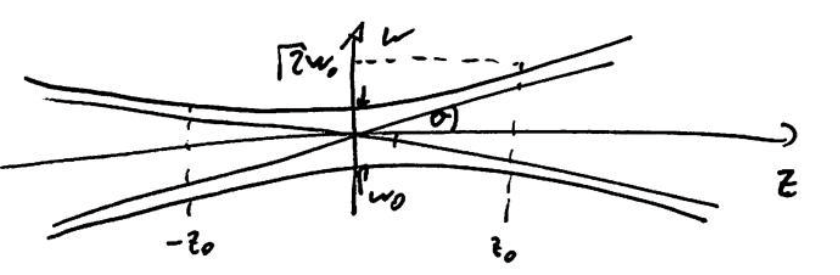
\includegraphics[width=\textwidth]{\currfiledir sketches/gauss_divergence.png}
   \caption{Divergence of a Gaussian beam}
\end{marginfigure}


We can define a \emph{divergence}, or opening angle $\Theta$ of the Gaussian beam. Far away from the beam waist, i.e. $z \ll z_0$ we have
\begin{equation}
    W(z) \approx W_0 \frac{z}{z_0} = \Theta \, z \quad \text{with} \quad \Theta = \frac{W_0}{z_0} = \frac{\lambda}{\pi W_0}
 \end{equation}
 Note that next to the wavelength $\lambda$ only the Rayleigh range $z_0$ \emph{or} the beam waist $W_0$ is a free parameter, not both. The divergence of the beam is fully contained in the beam waist. One can interpret this as diffraction of the Gaussian beam at its own waist. For comparison, diffraction at a circular aperture of radius $R$ would  lead to an angle $\Theta_\text{app} = 0.61 \lambda  / R$.

 \begin{figure}
    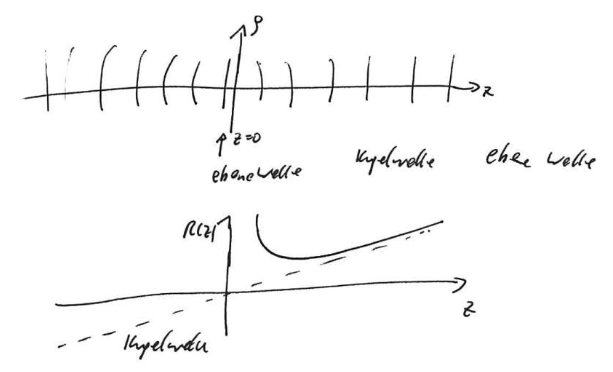
\includegraphics[width=\textwidth]{\currfiledir sketches/gauss_phase.png}
   \caption{Phase fronts and radius of curvature $R$ around the beam waist.}
\end{figure}

The phase of the Gaussian beam is given by the imaginary factors of the exponential function, i.e.
\begin{equation}
    \phi(\rho, z) = k z + k  \frac{\rho^2}{2 R(z)}  -  \zeta(z) 
\end{equation}
and the curvature of the phase fronts by 
\begin{equation}
    R(z) = z \left[ 1 + \left( \frac{z_0}{z} \right)^2 \right] 
\end{equation}
At the focus ($z=0$) and for $z \rightarrow \infty$ we find a diverging radius of curvature, i.e., a plane wave. For large distances this is the same as for a circular wave. Around the focus, the Gaussian beam differs as the radius of curvature changes such that we also get a plane wave exactly at $z=0$. Another peculairity of Gaussian beams is the \emph{Gouy phase} $\zeta(z)$
\begin{equation}
    \zeta(z) =  \arctan \frac{z}{z_0} 
\end{equation}
When passing through the focus, the wave undergoes a $pi$ phase shift. An intuitive picture could be the following\footcite{Boyd1980IntuitiveEO}: In geometrical optics, the ray would go through the focus. In a Gaussian beam, the path along the $1/e$ contour stays on the same side of the optical axis and in thus around the focus a bit shorter. This is compensated by the Gouy phase shift.


XXX M Parameter ??


\section{Gaussian beams as eigenmodes of a resonator}
The importance of Gaussian beams comes from the laser as a ubiquitous light source. A laser produces Gaussian beams because these wave functions are the eigenmodes of a resonator formed by two spherical mirrors.

In a laser, we are interested in eigenmodes, i.e. optical wave functions that do not change as they bounce back and forth in the resonator. The mirrors in a laser cavity are typically so highly reflective that there are many round trips before the field leaves the cavity.


\begin{marginfigure}
    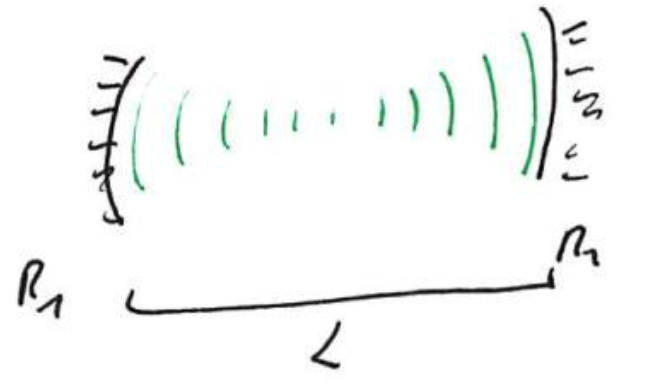
\includegraphics[width=\textwidth]{\currfiledir sketches/cavity.png}
   \caption{Eigenmodes of a laser cavity}
\end{marginfigure}


For an eigenmode to occur, the wavefront of the mode at the position of the mirror must match the shape of the mirror, otherwise it will reflect back into itself. The design of the cavity gives the radius of curvature $R_1$ and $R_2$ and the distance $d$ between the mirrors. We now show that under certain conditions a Gaussian beam is an eigenmode of such a cavity.

We search for the positions $z_1$ and $z_2$ of the mirrors and the Rayleigh range $z_0$ if the mean. We have the equation system
\begin{align}
    z_2 = & z_1 + d \\
    R_1 = & z_1 \left[ 1 + \left( \frac{z_0}{z_1} \right)^2 \right] \\
    R_2 = & z_2 \left[ 1 + \left( \frac{z_0}{z_2} \right)^2 \right] 
\end{align}

The solution is
\begin{align}
    z_1 = & \frac{-d (R_2 + d)}{R_1 + R_2 + 2d} \\
    z_2 = &z_1 + d  \\
    z_0^2 = & \frac{-d (R_1 +d)(R_2 + d)(R_1 + R_2 +d)}{(R_1 + R_2 + 2d)^2}
\end{align}
For a Gaussian beam $z_0$ must be real (or $z_0^2 > 0$). Otherwise $q = z - i z_0$ would be real and we would get a paraboloidal wave. This results in the \emph{stability condition} of a spherical cavity
\begin{equation}
    0 \le \left( 1 + \frac{d}{R_1} \right) \left( 1 + \frac{d}{R_2} \right) \le 1
\end{equation}

XXX sketch of stability condition

\section{Thin lens}

What happens when a Gaussian beam passes through a thin lens? We assume a thin lens, so $z$ does not change. The radial amplitude distribution $ \tilde{u}(\rho, z)$ also does not change, which means that the width parameter $W$ remains the same, i.e,
\begin{equation}
    W^{(L)} = W^{(R)}
\end{equation}
The phase needs a bit more attention. Just before the lens, the phase of the Gaussian beam is
\begin{equation}
   \phi^{(L)} =  k z + k  \frac{\rho^2}{2 R}  -  \zeta(z) 
\end{equation}
The phase effect of a lens is (see eq XXX)
\begin{equation}
  \Delta\phi_\text{lens} =   - k \frac{\rho^2}{2f}
\end{equation}
so that after the lens we have in total
\begin{equation}
  \phi^{(R)} =  \phi^{(L)}   + \Delta\phi_\text{lens}  =   k z   -  \zeta(z)  + k  \left( \frac{\rho^2}{2 R} - \frac{\rho^2}{2f} \right)
\end{equation}  
i.e. 
\begin{equation}
    \frac{1}{R^{(R)}} = \frac{1}{R^{(L)}} - \frac{1}{f}
\end{equation}

What does this mean for the other properties of a Gaussian beam? How are Rayleigh range $z_0$ and beam waits $W_0$ modified by a lens? Knowing $\lambda$, $W(z)$ and .$R$, i.e, the beam properties at the lens, we can use eqs XXX to calculate $z_0$, $W_0$ and $z$, i.e. the focal parameter and the distance $z$ of focus and lens. We get
\begin{align}
    W_0 = & \frac{W(z)}{\sqrt{1 + \left(\frac{\pi W(z)}{ \lambda R(z)} \right)^2}} \\
    z = & \frac{R(z)}{1 + \left(\frac{\pi W(z)}{ \lambda R(z)} \right)^2}
\end{align}
We thus can connect the left and right beam parameters.



\begin{figure}
    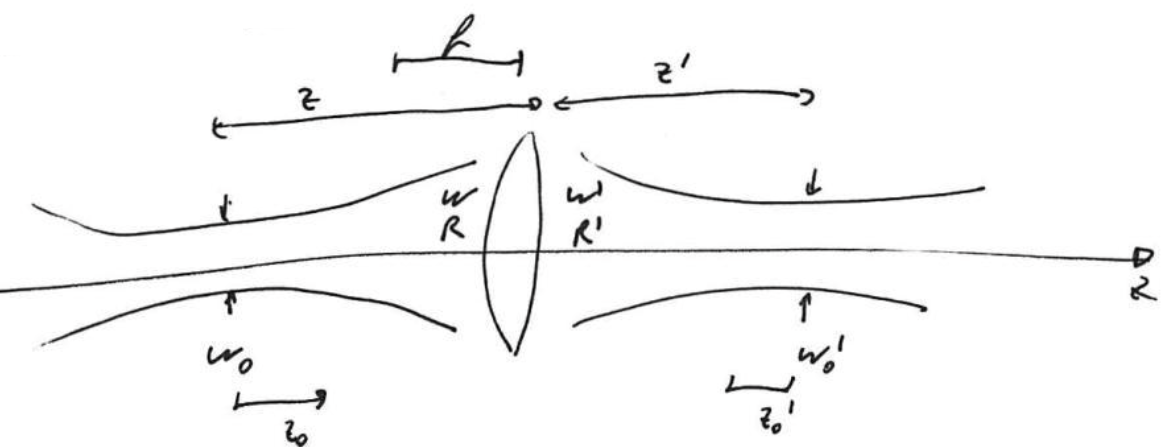
\includegraphics[width=\textwidth]{\currfiledir sketches/gauss_lens.png}
   \caption{A lens acting on a Gaussian beam}
\end{figure}


When the left beam waist is far from the lens, then we can see this arrangement as imaging of the left beam waist to a position $z^{(R)}$ on the right side  of the lens, which will magnify the beam waist radius. The magnification factor in ray optics is 
\begin{equation}
    M_r = \left| \frac{f}{z^{(L)} -f}  \right| \quad \text{and} \quad W_0^{(R)} \approx M_r W_0^{(L)} 
\end{equation}
The requirement 'far enough' means $z^{(L)} - f \gg z_0^{(L)} $, or
\begin{equation}
    r = \frac{z_0^{(L)} }{z^{(L)}  - f} \ll 1
\end{equation}
We can calculate the beam parameters without  this approximation using a general magnification factor $M$ and obtain
\begin{align}
    M = & \frac{M_r}{\sqrt{1 + r^2}} \\
    W_0^{(R)}  = & M W_0^{(L)}  \\
    (z^{(R)} - f) = &M^2 (z^{(L)} -f) \\
    z_0^{(R)} = & M^2 z_0^{(L)}  \\
    \Theta_0^{(R)} = & \frac{\Theta_0^{(L)} }{M}
\end{align}

\section{ABCD Law and q parameter}

Things become simpler when we realize that the $q$ parameter is governing the Gaussian beam. We introduced above the Gaussian beams by 
\begin{equation}
    q(z) = z - i z_0 \quad \text{and} \quad
    \frac{1}{q(z)} = \frac{1}{R(z)} + i \frac{\lambda}{\pi W^2(z)}
\end{equation} 
As soon as we know $q$ at a single position along the beam, we can calculate all the rest. When $q_1$  and $q_2$ describe the $q$ parameters left and right of an optical element, both are connected by the \emph{ABCD law}
\begin{equation}
    q_2 = \frac{A q_1 + B}{C q_1 + D}
\end{equation}
where 
\begin{equation}
\boldsymbol{M} = 
\begin{pmatrix}
    A & B \\ C & D \\
\end{pmatrix}
\end{equation}
is the $2\times2$ matrix of the matrix method in ray optics, as introduced in the last chapter.\sidenote{see \cite{Brooker_Optics}, chapter 7.9, for a justification.}

\emph{Propagation} by a distance $d$ thus leads to 
\begin{equation}
    q_2 = q_1 + d
\end{equation}
The action of a \emph{lens} is described by
\begin{equation}
    q_2 = \frac{f q_1}{f - q_1}
\end{equation}


%\section{Bonus: Hermit- and Laguerre-Gaussian beams}


\section{Technique: Knife Edge Test}


A common tool for determining the properties of a Gaussian beam is a knife edge or razor blade. We mount it so that it can be moved perpendicular to the optical axis, cutting out a variable part of the beam. If we measure the power in the beam after the knife edge as a function of its position, we get a partial integral over the cross-section of the beam.
\begin{equation}
    P(x_0) = \int_{x=x_0}^\infty \int_{y=-\infty}^\infty I(x,y) \, dx \, dy
\end{equation}
Taking the numerical derivative yields the beams intensity profile.
\begin{equation}
    I(x) \propto \frac{\partial P(x_0)}{\partial x_0}
\end{equation}


We can also observe the shadow of the knife edge to determine the position of the beam waist. We place a screen far from the waist and the knife edge at the estimated waist position. If the knife is between the waist and the screen, the shadow will start from the same side as the knife enters the beam. If the knife is further away than the waist, the directions are reversed. If the knife is exactly at the waist, the image on the screen will turn dark with no apparent direction. This is the \emph{Foucault knife edge test} to determine the position and quality of a focus, originally of a spherical mirror.

\begin{questions}
    \item Explain why the image turns dark with no apparent direction.
\end{questions}

%--------------------
\printbibliography[segment=\therefsegment,heading=subbibliography]
